\documentclass{beamer}
\usetheme{Goettingen}%Warsaw}
\usepackage[utf8]{inputenc}
\date{18th March 2011}
\author{Samuel Marpaux -- Philippe Pittoli}
\title[Nvidia]{English presentation -- Nvidia}
\begin{document}

\frame{
	\titlepage{NVIDIA}
}
\frame{
	\frametitle{Table of contents}
	\tableofcontents[pausesections]
}

\section{Introduction}
\subsection{The company}
\begin{frame}{Presentation of NVIDIA}
	\transdissolve[duration=0.03]

	\begin{block}{Founded}
		\begin{itemize}
			\item<+->{1993}
		\end{itemize}
	\end{block}	
	\pause
	\begin{block}{Location of head office}
		\begin{itemize}
			\item<+->{Santa Clara, California}
		\end{itemize}
	\end{block}
	\pause
	\begin{block}{Employees}
		\begin{itemize}
			\item<+->{~5,700}
			\item<+->{In more than 20 countries}
		\end{itemize}
	\end{block}
\end{frame}

\begin{frame}{Presentation of NVIDIA}
	\transdissolve[duration=0.08]
	\begin{block}{Localisation of head office}
	\begin{figure}[h]
		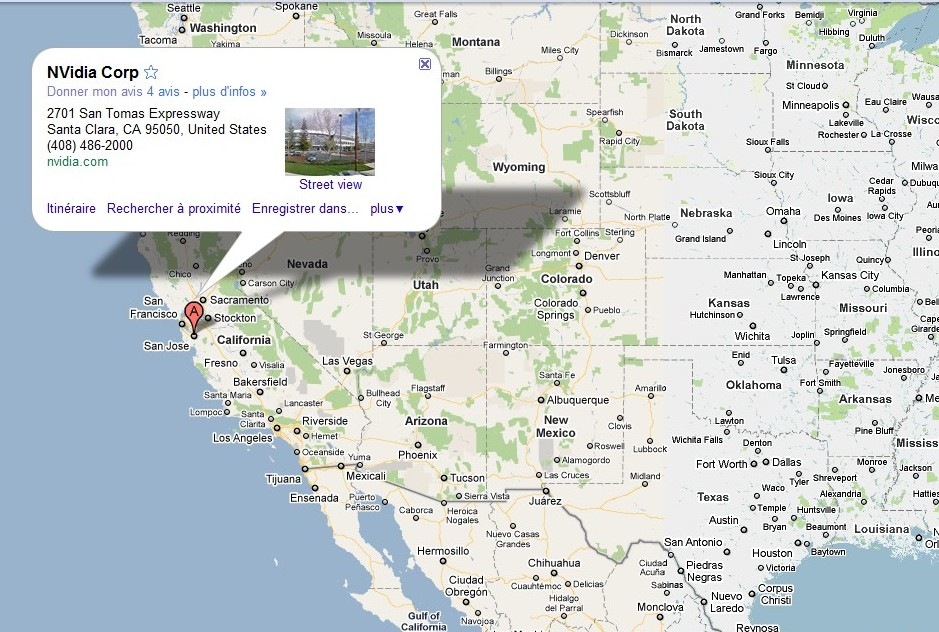
\includegraphics[width=1.05\textheight]{nvidiamap.jpg}
	\end{figure}
	\end{block}
\end{frame}

\begin{frame}{Presentation of NVIDIA}
	\transdissolve[duration=0.08]
	\begin{itemize}
		\item<+->{Headquarters}
	\end{itemize}
	\begin{figure}[h]
		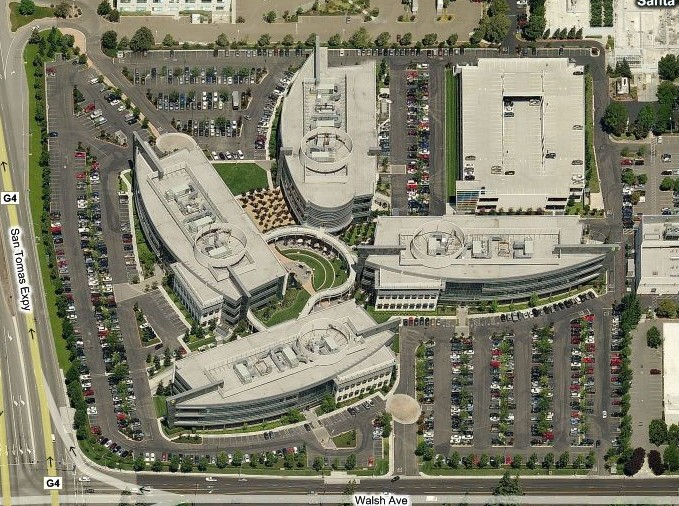
\includegraphics[width=1.00\textheight]{nvidia_locaux.jpg}
	\end{figure}
\end{frame}

\begin{frame}{Presentation of NVIDIA}
	\transdissolve[duration=0.08]
	\begin{itemize}
		\item<+->{Headquarters}
	\end{itemize}
	\begin{figure}[h]
		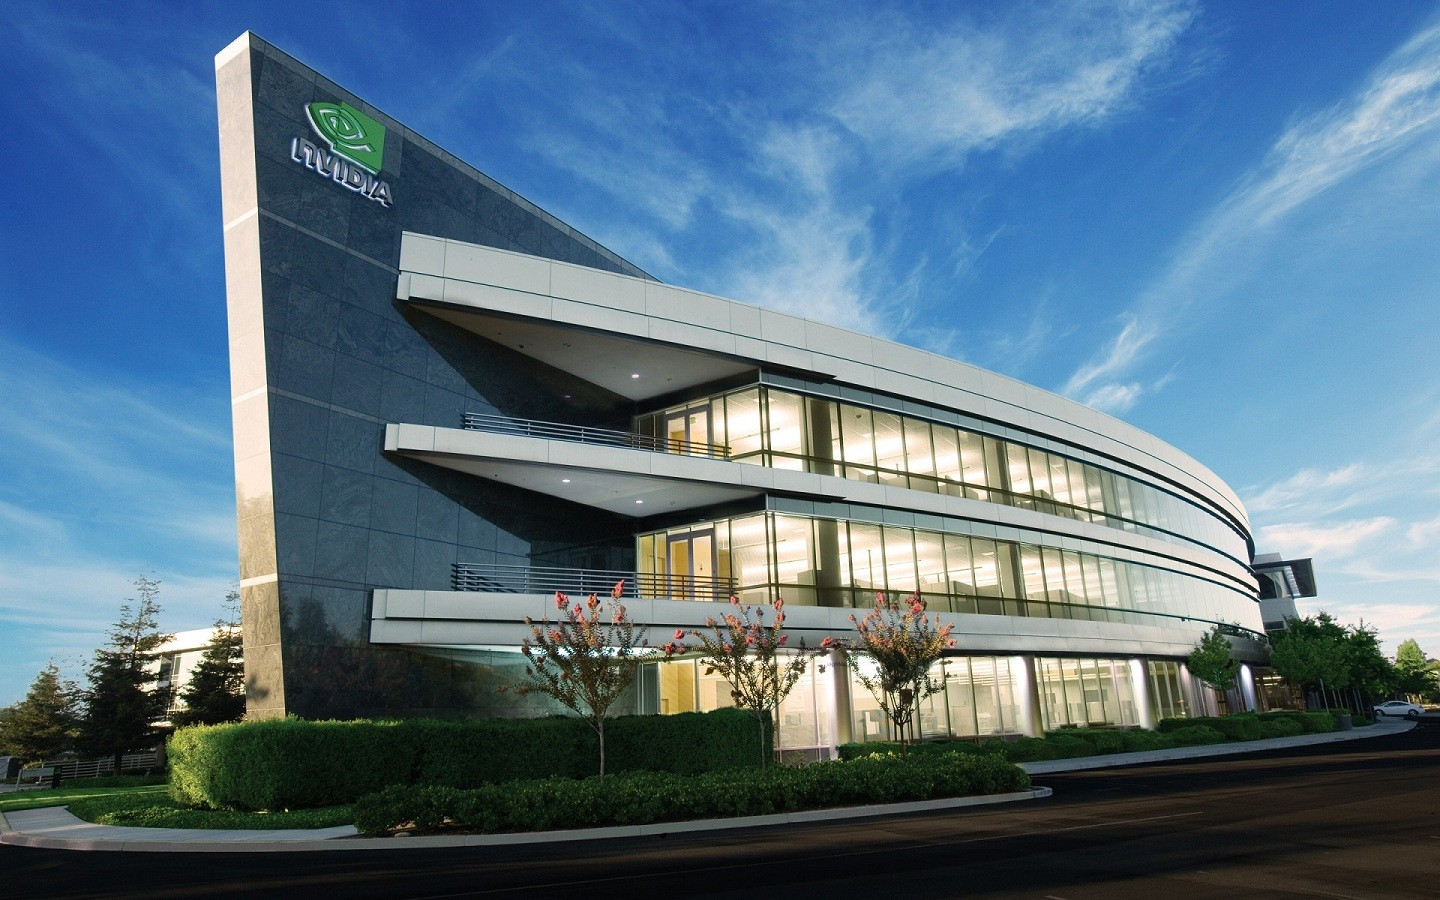
\includegraphics[width=1.00\textheight]{NVIDIA_HEADQUARTERS.jpg}
	\end{figure}
\end{frame}


\begin{frame}{Presentation of NVIDIA}
	\begin{block}{Funders}
		\begin{itemize}
			\item<+->{Jen-Hsun Huang -- CEO}
			\item<+->{Chris Malachowsky -- Senior Vice President}
			\item<+->{Curtis Priem -- Chief Technology Officer (retired)}
			\item<+->{Dr. Ranga Jayaraman -- Chief Information Officer}
		\end{itemize}
	\end{block}

\end{frame}

\begin{frame}{Presentation of NVIDIA}
	\transdissolve[duration=0.08]
	\begin{block}{}
		\begin{itemize}
			\item<+->{Jen-Hsun Huang}
		\end{itemize}
	\end{block}
	\begin{figure}[h]
		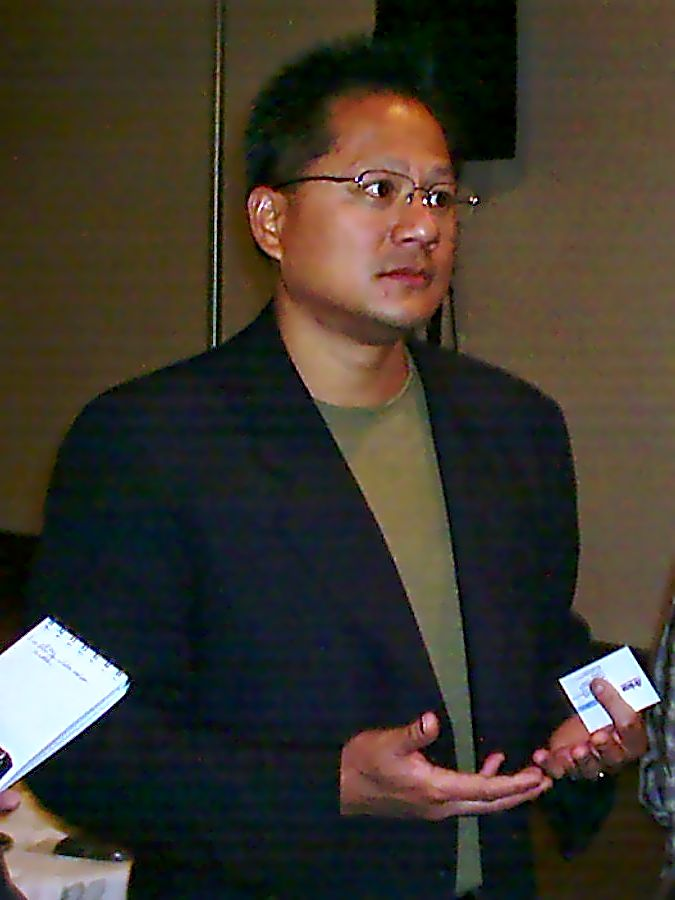
\includegraphics[width=0.50\textheight]{JensenHuang.jpg}
	\end{figure}
\end{frame}

\subsection{Work conditions}
\begin{frame}{Work conditions - Pros}

	\begin{block}{Health Care Benefits}
		\begin{itemize}
			\item<+->{Medical}
			\item<+->{Dental}
			\item<+->{Vision}
		\end{itemize}
	\end{block}
	\begin{block}{Financial Benefits}
		\begin{itemize}
			\item<+->{Pre-Tax Premiums}
			\item<+->{401(k) Retirement Plan}
			\item<+->{Flexible Spending Accounts (FSAs)}
			\item<+->{Discounts and special promotions}
		\end{itemize}
	\end{block}
\end{frame}
\begin{frame}{Work conditions - Pros}
	\begin{block}{Miscellaneous}
		\begin{itemize}
			\item<+->{Subsidized cafe}
			\item<+->{Laundry and dry cleaning}
			\item<+->{On-site Chair Massages}
			\item<+->{Even On-site Haircuts !}
		\end{itemize}
	\end{block}
\end{frame}

\begin{frame}{Work conditions - Cons}
	\begin{block}{According to an employee}
		\begin{itemize}
			\item<+->{No 401(k) matching}
			\item<+->{No free lunches}
			\item<+->{No discount on company products}
		\end{itemize}
	\end{block}
\end{frame}

\subsection{Partners}
\begin{frame}{Its Partners}
	\begin{block}{The partners}
		\begin{itemize}
			\item<+->{ASUS}
			\item<+->{EVGA}
			\item<+->{Gigabyte}
			\item<+->{PNY}
			\item<+->{Zotac}
			\item<+->{etc.}
		\end{itemize}
	\end{block}
\end{frame}

\section{Products}
\subsection{Hardwares}
\begin{frame}{The Nvidia products}
	\transdissolve[duration=0.1]
	\begin{block}{The main products}
		\begin{itemize}
			\item<+->{PC video-cards}
			\item<+->{Motherboard chipsets}
		\end{itemize}
	\end{block}
\end{frame}
\begin{frame}{The other products}
	\transdissolve[duration=0.1]
	\begin{block}{state-of-the-art hardwares}
		\begin{itemize}
			\item<+->{dedicated GPGPU processors (TESLA)}
			\item<+->{Tegra: system-on-a-chip}
		\end{itemize}
	\end{block}
	\begin{block}{GPUs for game consoles}
		\begin{itemize}
			\item<+->{Xbox : GeForce3-class GPU (on an Intel Pentium III/Celeron platform)}
			\item<+->{PlayStation 3 : RSX 'Reality Synthesizer'}
		\end{itemize}
	\end{block}
\end{frame}

\subsection{Softwares}
\begin{frame}{The NVIDIA technologies}
	\transdissolve[duration=0.1]
	\begin{block}{Pioneers in different technologies}
		\begin{itemize}
			\item<+->{SLI}
			\item<+->{CUDA}
			\item<+->{PhysX}
			\item<+->{OpenCL}
			\item<+->{and many others}
		\end{itemize}
	\end{block}
\end{frame}

\section{Competitors}
\begin{frame}{The competitors}
	\transdissolve[duration=0.1]
	\begin{block}{}
		\begin{itemize}
			\item<+->{AMD, Advanced Micro Devices \\(formerly ATI Technologies Inc.)}
		\end{itemize}

		\begin{itemize}
			\item<+->{Intel, Integrated Electronics}
			\begin{itemize}
				\item<+->{Only on motherboard chipset market}
			\end{itemize}
		\end{itemize}
	\end{block}
\end{frame}

\section{Company Data}
\subsection{Figures}
\begin{frame}{Figures}
	\transdissolve[duration=0.1] % Crée un effet => Turnover s'affiche mais l'item dans le bloc ne s'affiche que plus tard
	\begin{block}{PC video-card gaming market share}
		\begin{itemize}
			\item<+->{NVIDIA : 59\% }
			\item<+->{AMD : 33\% }
		\end{itemize}
	\end{block}	
	\begin{block}{2010 - Turnover (in M \$)}
		\begin{itemize}
			\item<+->{~3,300}
		\end{itemize}
	\end{block}
	\begin{block}{2010 - Net income (in M \$)}
		\begin{itemize}
			\item<+->{-68}
		\end{itemize}
	\end{block}
\end{frame}

\subsection{Graphs}
\begin{frame}{Graphs}
	\begin{block}{Income - Statement - Evolution}
		\begin{figure}[h]
			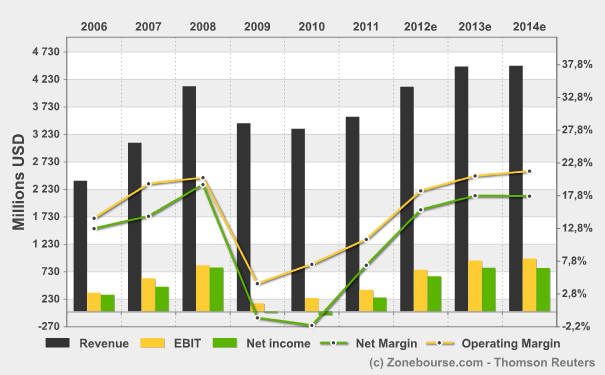
\includegraphics[width=0.90\textheight]{./Income_Statement_Evolution.png}
		\end{figure}
	\end{block}	
\end{frame}
\begin{frame}{Graphs}
	\begin{block}{Annual Income Statement Data}
		\begin{figure}[h]
			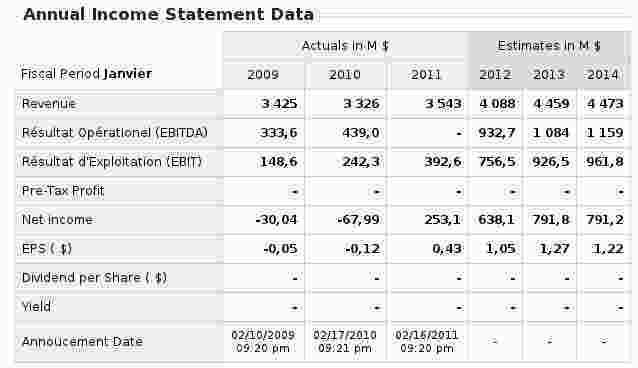
\includegraphics[width=0.90\textheight]{./Annual_Income_SD_NVIDIA.jpeg}
		\end{figure}
	\end{block}	
\end{frame}
\begin{frame}{Graphs}
	\begin{block}{In comparison with AMD}
		\begin{figure}[h]
			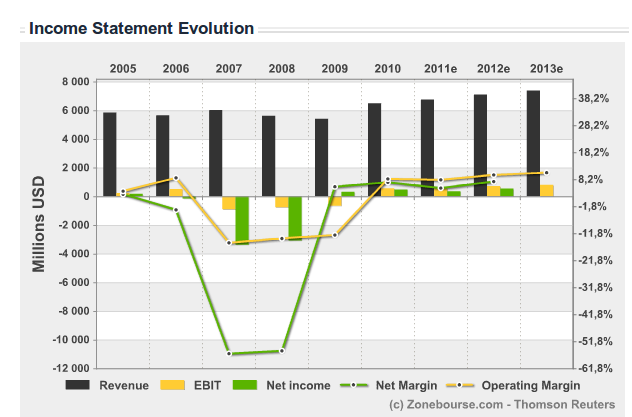
\includegraphics[width=0.90\textheight]{./Income_Statement_Evolution_amd.png}
		\end{figure}
	\end{block}	
\end{frame}

\end{document}
